\documentclass[a4paper,twocolumn,10pt]{article}
\usepackage[margin=25mm,left=20mm,right=20mm]{geometry}
\usepackage{graphicx}
\usepackage{booktabs}
\usepackage{times}
\pagestyle{empty}
\setlength{\columnsep}{10mm}
\title{\textbf{FPGA Implementation of a PatchCore-lite Anomaly Detection System with Category-wise Profile Switching}}
\author{Shunya Yamada and Kazuyoshi Takagi\\ Computer Architecture Laboratory, Department of Information Engineering, Graduate School of Engineering, Mie University\\ (E-mail: shunya@arch.info.mie-u.ac.jp)}
\date{}
\begin{document}
\maketitle
\begin{abstract}
PatchCore is a strong industrial anomaly detection method that stores normal patch features in a memory bank and detects anomalies by k-nearest neighbor (KNN) search. However, a multi-product inspection line forces one common configuration to cover different object categories, increasing KNN search cost and making FPGA implementation memory-bound. This paper studies a PatchCore-lite system that keeps one shared CNN backbone but switches category-specific profiles, including the extracted feature layer, grid resolution, top-k score setting, threshold, and memory-bank address. Experiments on MVTec AD indicate that the proposed switching reduces the theoretical KNN search cost while preserving or improving the good-product pass rate under a fixed defect false-pass constraint.
\end{abstract}
\noindent\textbf{Keywords:} industrial anomaly detection, PatchCore, FPGA, KNN search, profile switching
\section*{1. INTRODUCTION}
Industrial visual inspection often needs high defect sensitivity and stable throughput. PatchCore [1] is attractive because it can be trained from normal samples only and has reported high image-level anomaly detection performance on MVTec AD [2]. Its main implementation cost is not back-propagation, but feature extraction and memory-bank KNN search.

A simple FPGA implementation can prepare one common profile and one common memory bank for all products. This is easy to control, but it searches unnecessary bank entries and uses one feature setting even when each product category has different visual characteristics. This study investigates whether product-category information, which is already known before inspection in many lines, can be used to select a lighter profile without reconfiguring the FPGA bitstream.

\section*{2. PATCHCORE}
PatchCore is an anomaly detection method based on normal feature memory. The training and inference flow is shown in Fig. 1. First, a backbone CNN extracts intermediate feature maps from an input image. These feature maps are converted into patch-level feature vectors. During training, feature vectors obtained only from normal images are stored as a memory bank. During inference, each input patch feature is compared with the memory bank by KNN search. If the input feature is far from the stored normal features, the image is judged anomalous.

The main design parameters are the backbone CNN, the feature profile, and the memory bank. The backbone CNN, such as WideResNet50-2, extracts feature maps from the image. A profile is the set of lightweight choices after this CNN: layer2/layer3 indicate which intermediate CNN feature maps are used, grid 14 means that the feature map is sampled into 14 x 14 patch positions, D is the feature-vector dimension per patch, and top-k is the fraction of the largest patch anomaly scores used to form the image anomaly score.

The memory bank stores representative normal patch features. A larger bank improves coverage of the normal distribution but increases memory traffic and KNN operations. k-center coreset selection is a standard technique that keeps representative bank entries while reducing the bank size [3]. To isolate the effect of category-wise profile switching, all compared systems use the same coreset-based bank budget in the main evaluation.

\begin{figure}[h]
\centering
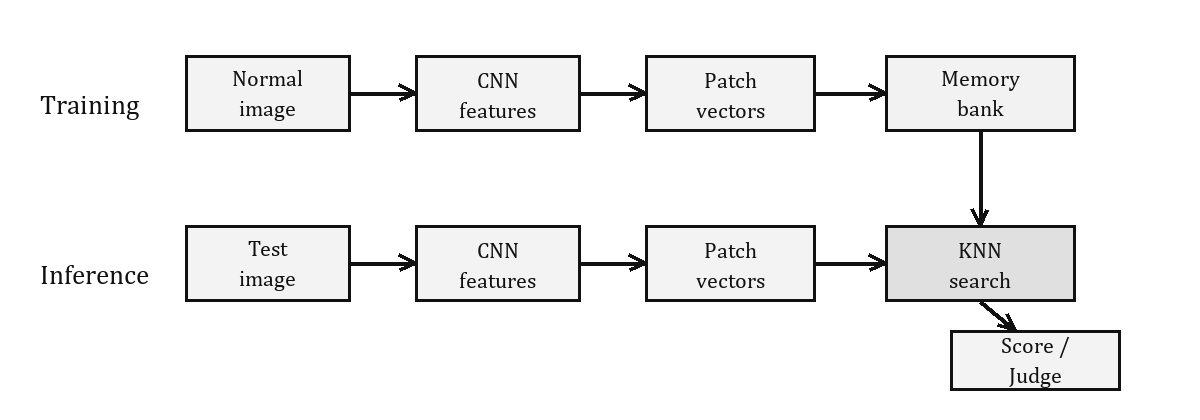
\includegraphics[width=\columnwidth]{figures/patchcore_process.png}
\caption{PatchCore training and inference flow.}
\end{figure}
\section*{3. PROPOSED SYSTEM}
The proposed system targets multi-category inspection on one FPGA, as illustrated in Fig. 2. It keeps one shared CNN datapath and switches only category-dependent profile registers and memory-bank ranges before inference. The switched parameters are feature layer, grid size, feature dimension, top-k aggregation, anomaly threshold, and the base address and search length of the category memory bank.

The proposed contribution is category-wise execution control in addition to conventional memory-bank reduction. Existing PatchCore acceleration commonly uses coreset selection to reduce stored features. The proposed system further uses product-category information, which is available before inspection, to select the feature profile and bank range used for the current product. This reduces active KNN search compared with a common multi-category PatchCore, while reusing the CNN and KNN datapath instead of preparing independent engines for each category.

\begin{figure}[h]
\centering
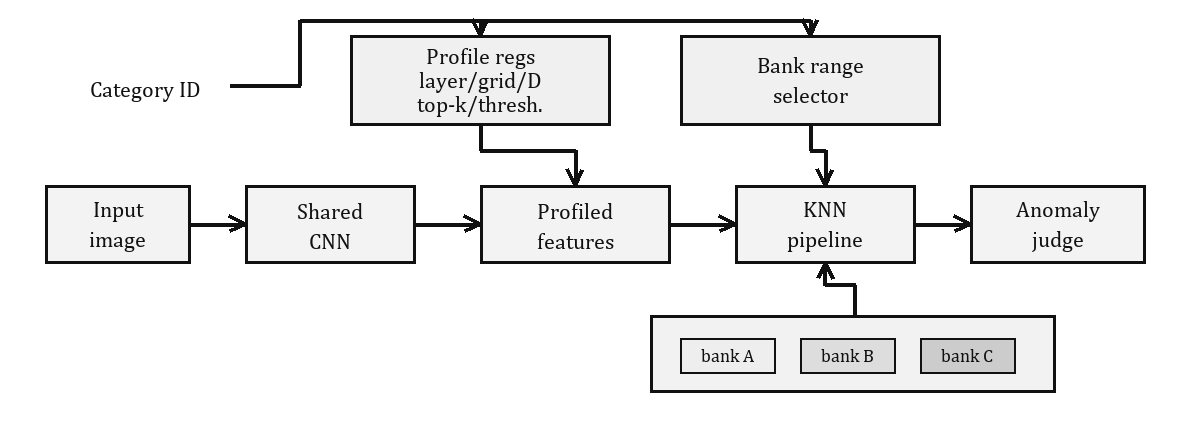
\includegraphics[width=\columnwidth]{figures/system_architecture.png}
\caption{Category-wise profile switching architecture.}
\end{figure}
\section*{4. EXPERIMENTAL SETUP}
Experiments used all 15 MVTec AD categories: bottle, cable, capsule, carpet, grid, hazelnut, leather, metal\_nut, pill, screw, tile, toothbrush, transistor, wood, and zipper. All two-category and three-category subsets were evaluated, giving 105 AB tasks and 455 ABC tasks, 560 tasks in total. Only normal training images were used to construct the memory bank, and both normal and defective test images were used for evaluation. The feature extractor was a PatchCore-like WideResNet50-2 backbone. The main comparison used k-center coreset selection with the same bank budget, bank/category = 3000, for all compared systems.

The evaluated metric was the good-product pass rate under a defect false-pass constraint of 3\% or lower. The defect false-pass rate is the fraction of defective samples judged normal. The good-product pass rate is the fraction of normal samples judged normal. The anomaly threshold was selected for each evaluated system so that the defect false-pass constraint was satisfied.

The compared systems were: (i) default profile with a common bank, (ii) default profile with category-bank switching, (iii) one category-specific profile fixed and applied to all categories with category-bank switching, and (iv) category-specific profile and category-bank switching. For (iii), the fixed profile with the highest mean good-product pass rate was selected for each subset, giving a strong single-profile baseline. The default profile was layer2+3, grid 14, D=768, and top-k fraction 0.010. Category-specific profiles were obtained before the subset experiment by a single-category sweep at bank=12000. For each category, profiles whose good-product pass rate was within 2 percentage points of the default profile under the 3\% defect false-pass constraint were kept, and the smallest profile by patch\_count x D was selected. The selected profiles are listed in Table 1.

\begin{table}[h]\centering\small
\caption{Category-specific profiles selected by single-category sweep.}
\begin{tabular}{lcccl}\toprule Layer & Grid & D & top-k & Category\\\midrule
layer3 & 14 & 512 & 0.005 & bottle, carpet, hazelnut, leather\\
layer3 & 14 & 512 & 0.005 & metal\_nut, tile, zipper\\
layer3 & 14 & 512 & 0.010 & screw, transistor\\
layer3 & 14 & 512 & 0.020 & capsule\\
layer3 & 14 & 512 & 0.050 & cable\\
layer2+3 & 14 & 768 & 0.005 & grid\\
layer2+3 & 14 & 768 & 0.010 & pill, wood\\
layer2+3 & 14 & 768 & 0.050 & toothbrush\\
\bottomrule\end{tabular}\end{table}
\section*{5. RESULTS}
Tables 2 and 3 summarize the AB and ABC results. For the 105 two-category tasks, the proposed profile-and-bank switching achieved 85.53\% mean good-product pass rate with 0.378x relative KNN search cost. For the 455 three-category tasks, it achieved 85.53\% with 0.252x relative cost. Thus, the proposed system maintained good-product pass performance while reducing the active search work, especially when more categories shared one inspection system.

Large improvements were observed in subsets where the common profile did not fit all categories well. In the cable+carpet task, the mean good-product pass rate increased from 52.59\% to 79.99\%, while the KNN search cost became 0.333x. In the cable+carpet+screw task, it increased from 37.99\% to 66.33\%, while the cost became 0.222x.

\begin{table}[h]\centering\small
\caption{Statistics for 105 AB tasks at <=3\% defect false-pass rate.}
\begin{tabular}{lccc}\toprule System & Mean good & Min good & KNN cost\\\midrule
Common profile + common bank & 80.27\% & 69.30\% & 1.000x\\
Category bank switch & 81.95\% & 71.73\% & 0.500x\\
Single fixed profile (best) & 85.01\% & 75.83\% & 0.400x\\
Proposed profile+bank switch & 85.53\% & 76.48\% & 0.378x\\
\bottomrule\end{tabular}\end{table}
\begin{table}[h]\centering\small
\caption{Statistics for 455 ABC tasks at <=3\% defect false-pass rate.}
\begin{tabular}{lccc}\toprule System & Mean good & Min good & KNN cost\\\midrule
Common profile + common bank & 79.27\% & 60.43\% & 1.000x\\
Category bank switch & 81.95\% & 65.44\% & 0.333x\\
Single fixed profile (best) & 84.49\% & 68.77\% & 0.271x\\
Proposed profile+bank switch & 85.53\% & 70.43\% & 0.252x\\
\bottomrule\end{tabular}\end{table}
\section*{6. DISCUSSION}
The results show an effect beyond memory-bank address switching. Category-bank switching reduced the search range, but the proposed system also improved the mean and minimum good-product pass rates by selecting the feature profile for each category. This indicates that useful feature layer, grid density, feature dimension, and top-k aggregation are category-dependent. For example, cable selected a larger top-k fraction, suggesting that categories with elongated structures or spatially distributed defects benefit from aggregating more high-score patches.

The fixed-profile baseline clarifies why switching is needed. Even when a strong single profile is selected for each subset, one category's profile is still forced onto the other categories. The proposed system avoids this profile mismatch by assigning each category its own profile before inspection. Thus, the contribution is stable category-specialized execution on a shared multi-category system.

The relative KNN search cost is modeled by Eq. (1). Since the main comparison fixes the bank budget per category, the additional reduction comes from profile parameters such as patch count and feature dimension. The lower relative cost in ABC tasks suggests that the benefit increases as the number of target categories increases.

\begin{equation}
C_m(S)=\sum_{c\in S}p_c P_{m,c}B_{m,c}D_{m,c},\quad R_m=\frac{C_m(S)}{C_{\rm common}(S)}
\end{equation}
\noindent where $P$, $B$, and $D$ denote patch count, searched bank size, and feature dimension.
\section*{7. FPGA COST ESTIMATE}
On FPGA, the reduction maps to bank base address, search length, feature-dimension enable, and profile registers. The system can reuse one CNN and KNN datapath while changing the active memory range and loop bounds for the current category.

Table 4 gives the FPGA-facing estimate. If 8-bit bank features and 64 distance lanes are assumed, KNN cycles and bank reads follow the relative KNN search cost. Under this model, the ABC result reduces KNN-side activity to about one quarter of the common-profile baseline.

The remaining evaluation is to implement the profile-controlled KNN pipeline and measure latency, memory bandwidth, logic usage, on-chip memory usage, and dynamic power. The KNN engine mainly scales with the number of distance lanes and memory ports, whereas category switching adds only profile registers, address offsets, and small multiplexers. The implementation will verify whether this switching overhead is smaller than the saved KNN loops and memory traffic.

\begin{table}[h]\centering\small
\caption{FPGA-facing estimate at bank/category=3000, 8-bit features, and 64 distance lanes.}
\begin{tabular}{lcccc}\toprule System & cycles/img & ratio & mem. & BRAM\\\midrule
Common profile+bank & 17.88M & 1.000x & 5.57MiB & 1267\\
Bank switch & 7.06M & 0.395x & 5.57MiB & 1267\\
Fixed profile+bank & 5.52M & 0.309x & 4.34MiB & 988\\
Proposed switch & 5.23M & 0.293x & 4.11MiB & 936\\
\bottomrule\end{tabular}\end{table}
\section*{8. CONCLUSION}
This study proposes category-wise profile switching for PatchCore-lite anomaly detection toward FPGA implementation. Experiments under a fixed defect false-pass constraint showed that profile switching can improve the good-product pass rate and reduce KNN search cost in multi-category inspection. The next step is FPGA implementation and measurement of the gap between the theoretical model and actual resource, latency, and power results.

\section*{REFERENCES}
\noindent [1] K. Roth, L. Pemula, J. Zepeda, B. Schoelkopf, T. Brox, and P. Gehler, "Towards Total Recall in Industrial Anomaly Detection," CVPR, pp. 14318-14328, 2022.\\
\noindent [2] P. Bergmann, M. Fauser, D. Sattlegger, and C. Steger, "MVTec AD--A Comprehensive Real-World Dataset for Unsupervised Anomaly Detection," CVPR, 2019.\\
\noindent [3] OpenVINO Anomalib Contributors, "PatchCore model documentation," 2026.\\
\end{document}